\chapter{Day 1}



\section{Mesh structure}

The general principle behind digital geometry processing is
approximating \emph{smooth manifolds} and the theory of
differential geometry regarding them to discrete scenarios.
We start by approximating manifolds and their properties.

\begin{marginfigure}
    \centering
    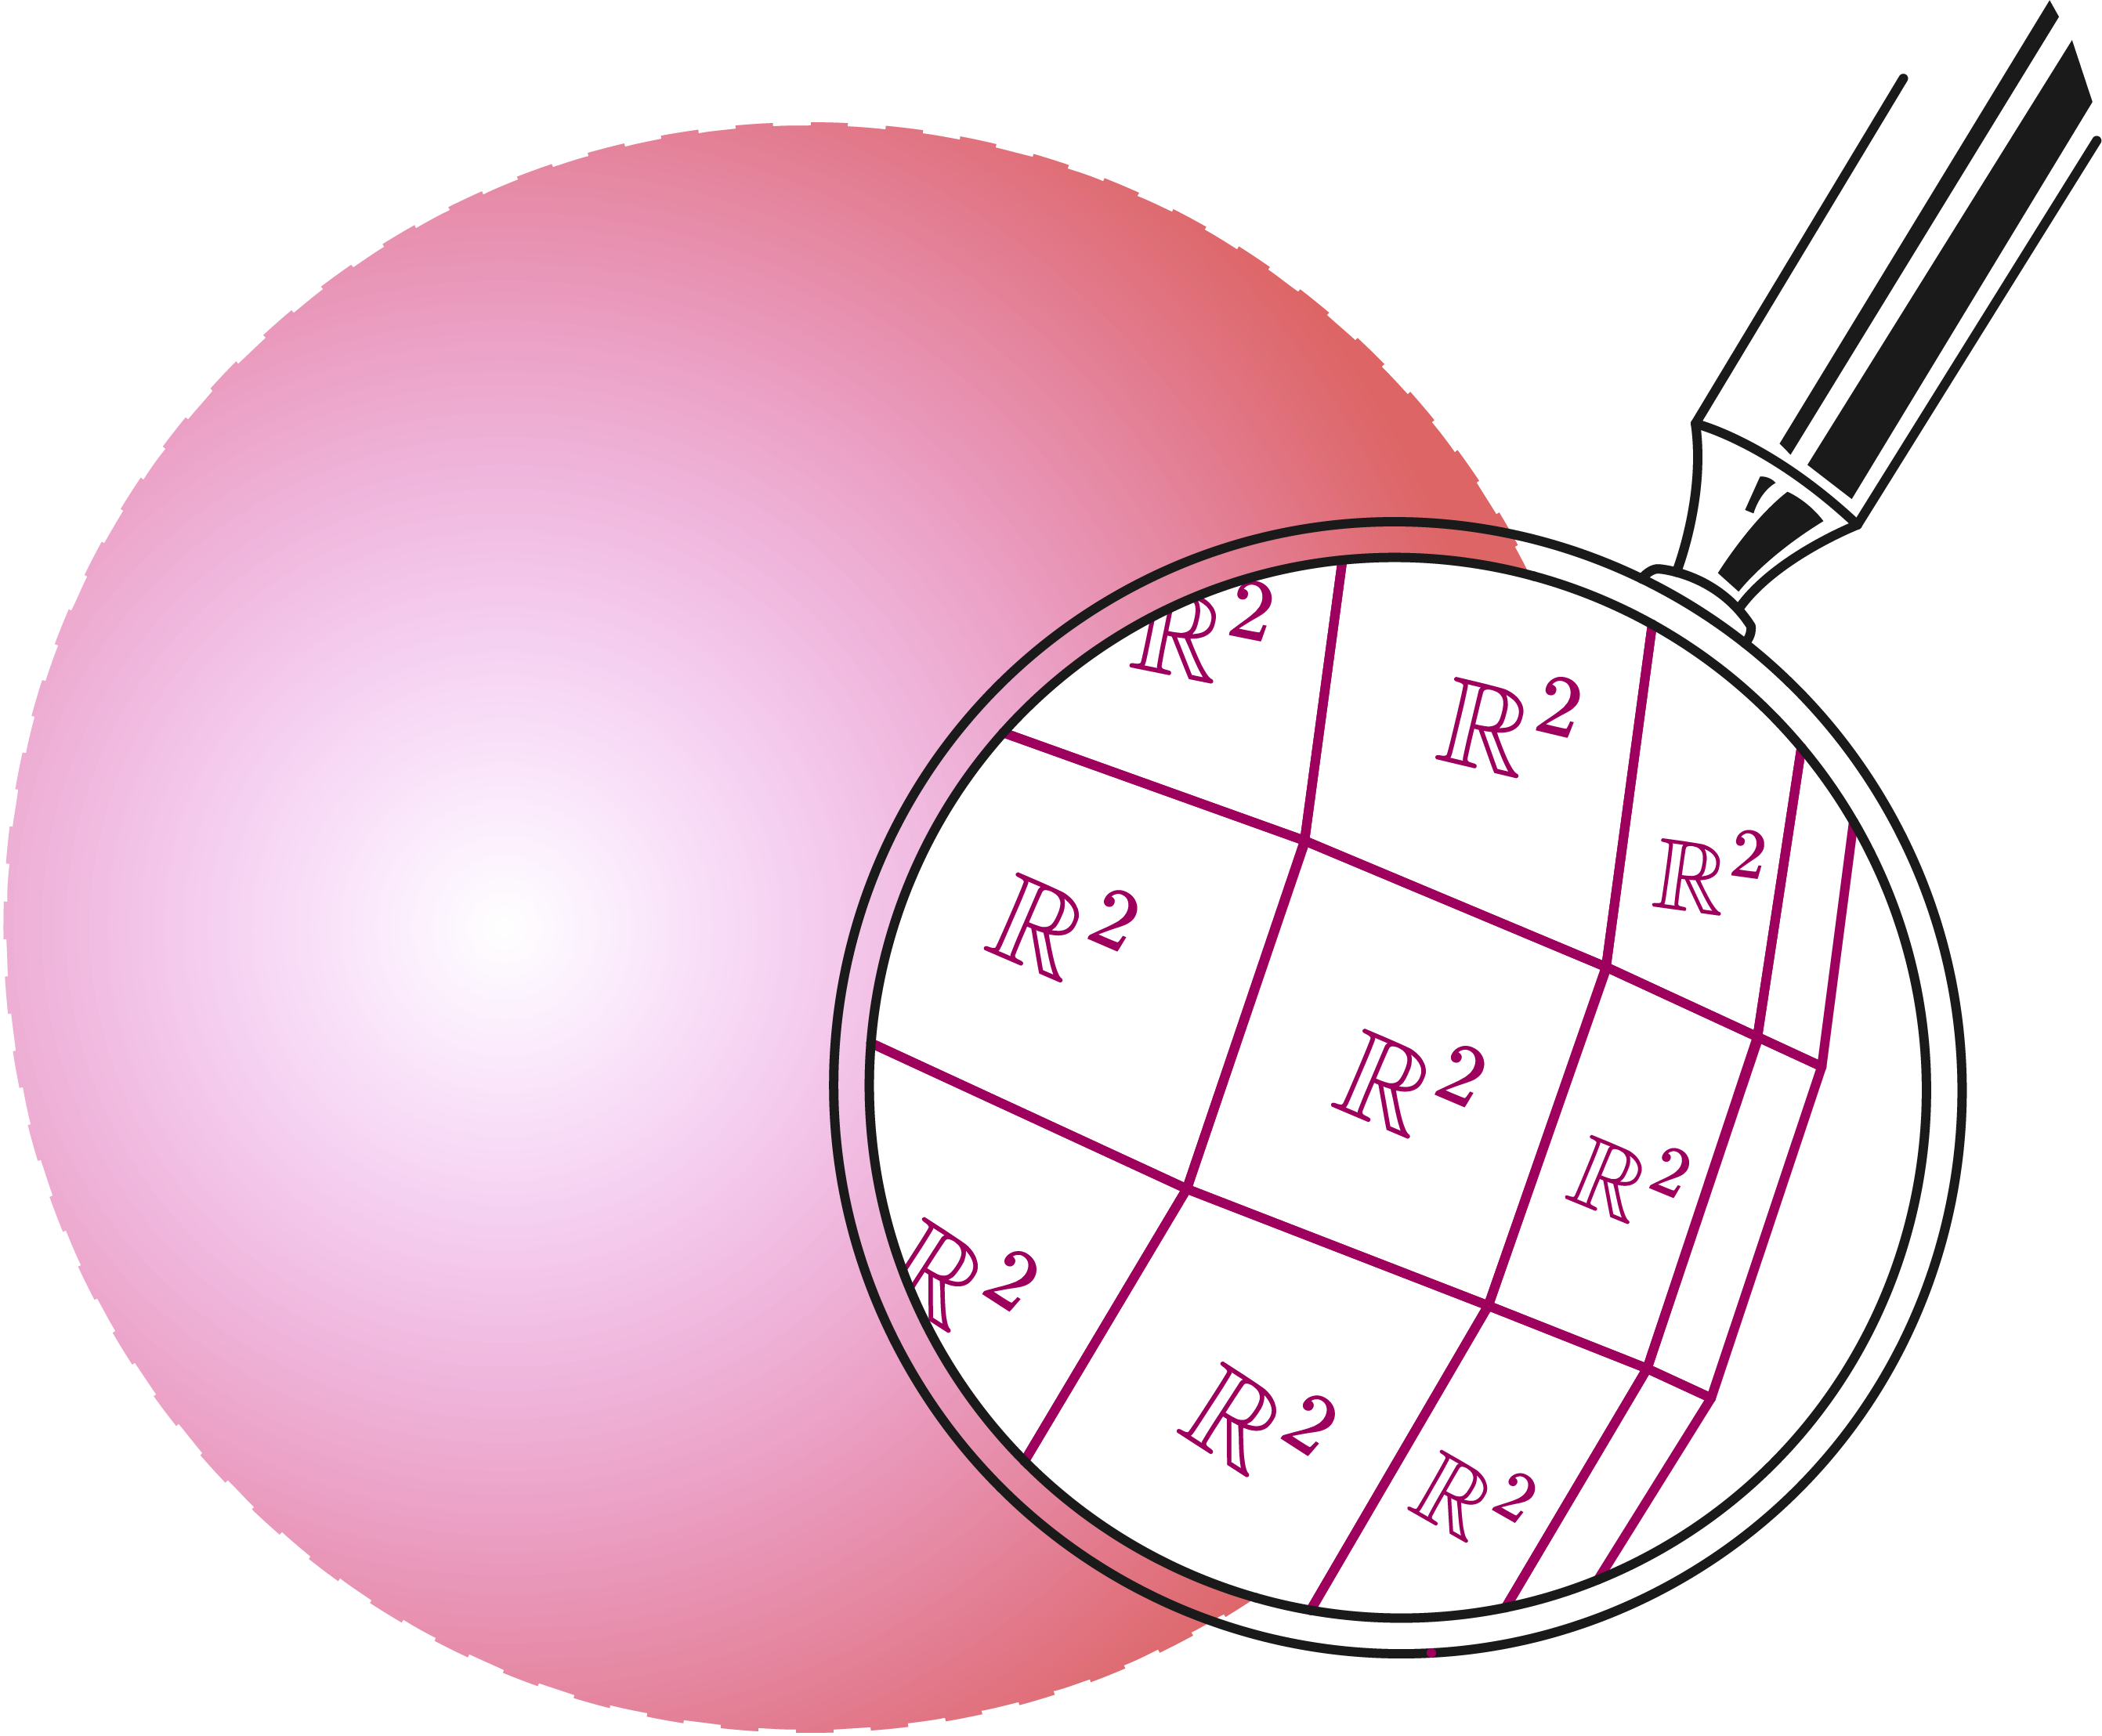
\includegraphics[width=0.8\linewidth]{images/sphere1.png}
    \caption{ A \textit{manifold} is a surface that under a microscope looks like
a flat sheet of paper, or $\RR^n$. Under the limit of 
infinite sheets of paper, you get a continous surface.}
\end{marginfigure}

\spa

A \textbf{\emph{mesh}} $\bf{M(V,E,F)}$ is a construction of some polygonal faces 
connected together, and the usual mesh is made up of rectangles or triangles 
stitched up together. You can make up the mesh by plotting the coordinates
of each of its vertices, at which point you get the
\emph{\textbf{vertex list}} $\Vsf \in  \RR^{n \times 3}$:

\begin{align*}
\begin{pmatrix}
\bf{v}^T_0\\
\bf{v}^T_1\\
\bf{v}^T_2 \\
\cdots
\end{pmatrix}
=
\begin{pmatrix}
x_0 &  y_0&  z_0\\
x_1 &  y_1&  z_1\\
x_2 &  y_2&  z_2 \\
&\cdots
\end{pmatrix}
=
\begin{pmatrix}
\text{1st Vertex}\\
\text{2nd Vertex}\\
\text{3rd Vertex}\\
\cdots
\end{pmatrix}
\end{align*}

Now, this gives us a nebulous little cloud of points. When you connect 
these little points together by some lines, you get \emph{edges} and a
\textit{\textbf{edge list}} $\bf{E}$;
get three of those in a loop, you get a \emph{face}. The faces of
the mesh compose a \emph{\textbf{face list}} $\bf{F}$. Therefore,
a mesh is composed of those three lists. \sidenote{One can also produce a
\textit{adjancency matrix} $\bf{A}$ \cite{benchen2010mesh} rather than
a edge connectivity list. This is related to how to inform directions in
planar graphs.}

\spa

In the same way as manifolds, lots of facts about algebraic and differential
topology can also be expressed for triangle meshes, namely 
topological invariants, which are numbers dependant only on the 
"qualitative characteristic" of the manifold at hand.
For example, per section 16.4.3 of \cite{realtime}, there is a very useful 
rule of thumb for roughly how many vertices, edges and faces a given triangular 
mesh will have, using the \emph{Euler-Poincaré formula} gives us
the \textit{Euler Characteristic} $\chi$:
\sidenote{A proof of this formula can be found in \cite{eulerpoincare1}}

\begin{definition}[Euler-Poincaré characteristic of a mesh]
    \begin{align*}
    \text{(Vertices) - (Edges)} + 2\text{(Faces) - (Loops)} + 2\text{(Genus)} = 2
\end{align*}
\end{definition}

\begin{marginfigure}
    \centering
    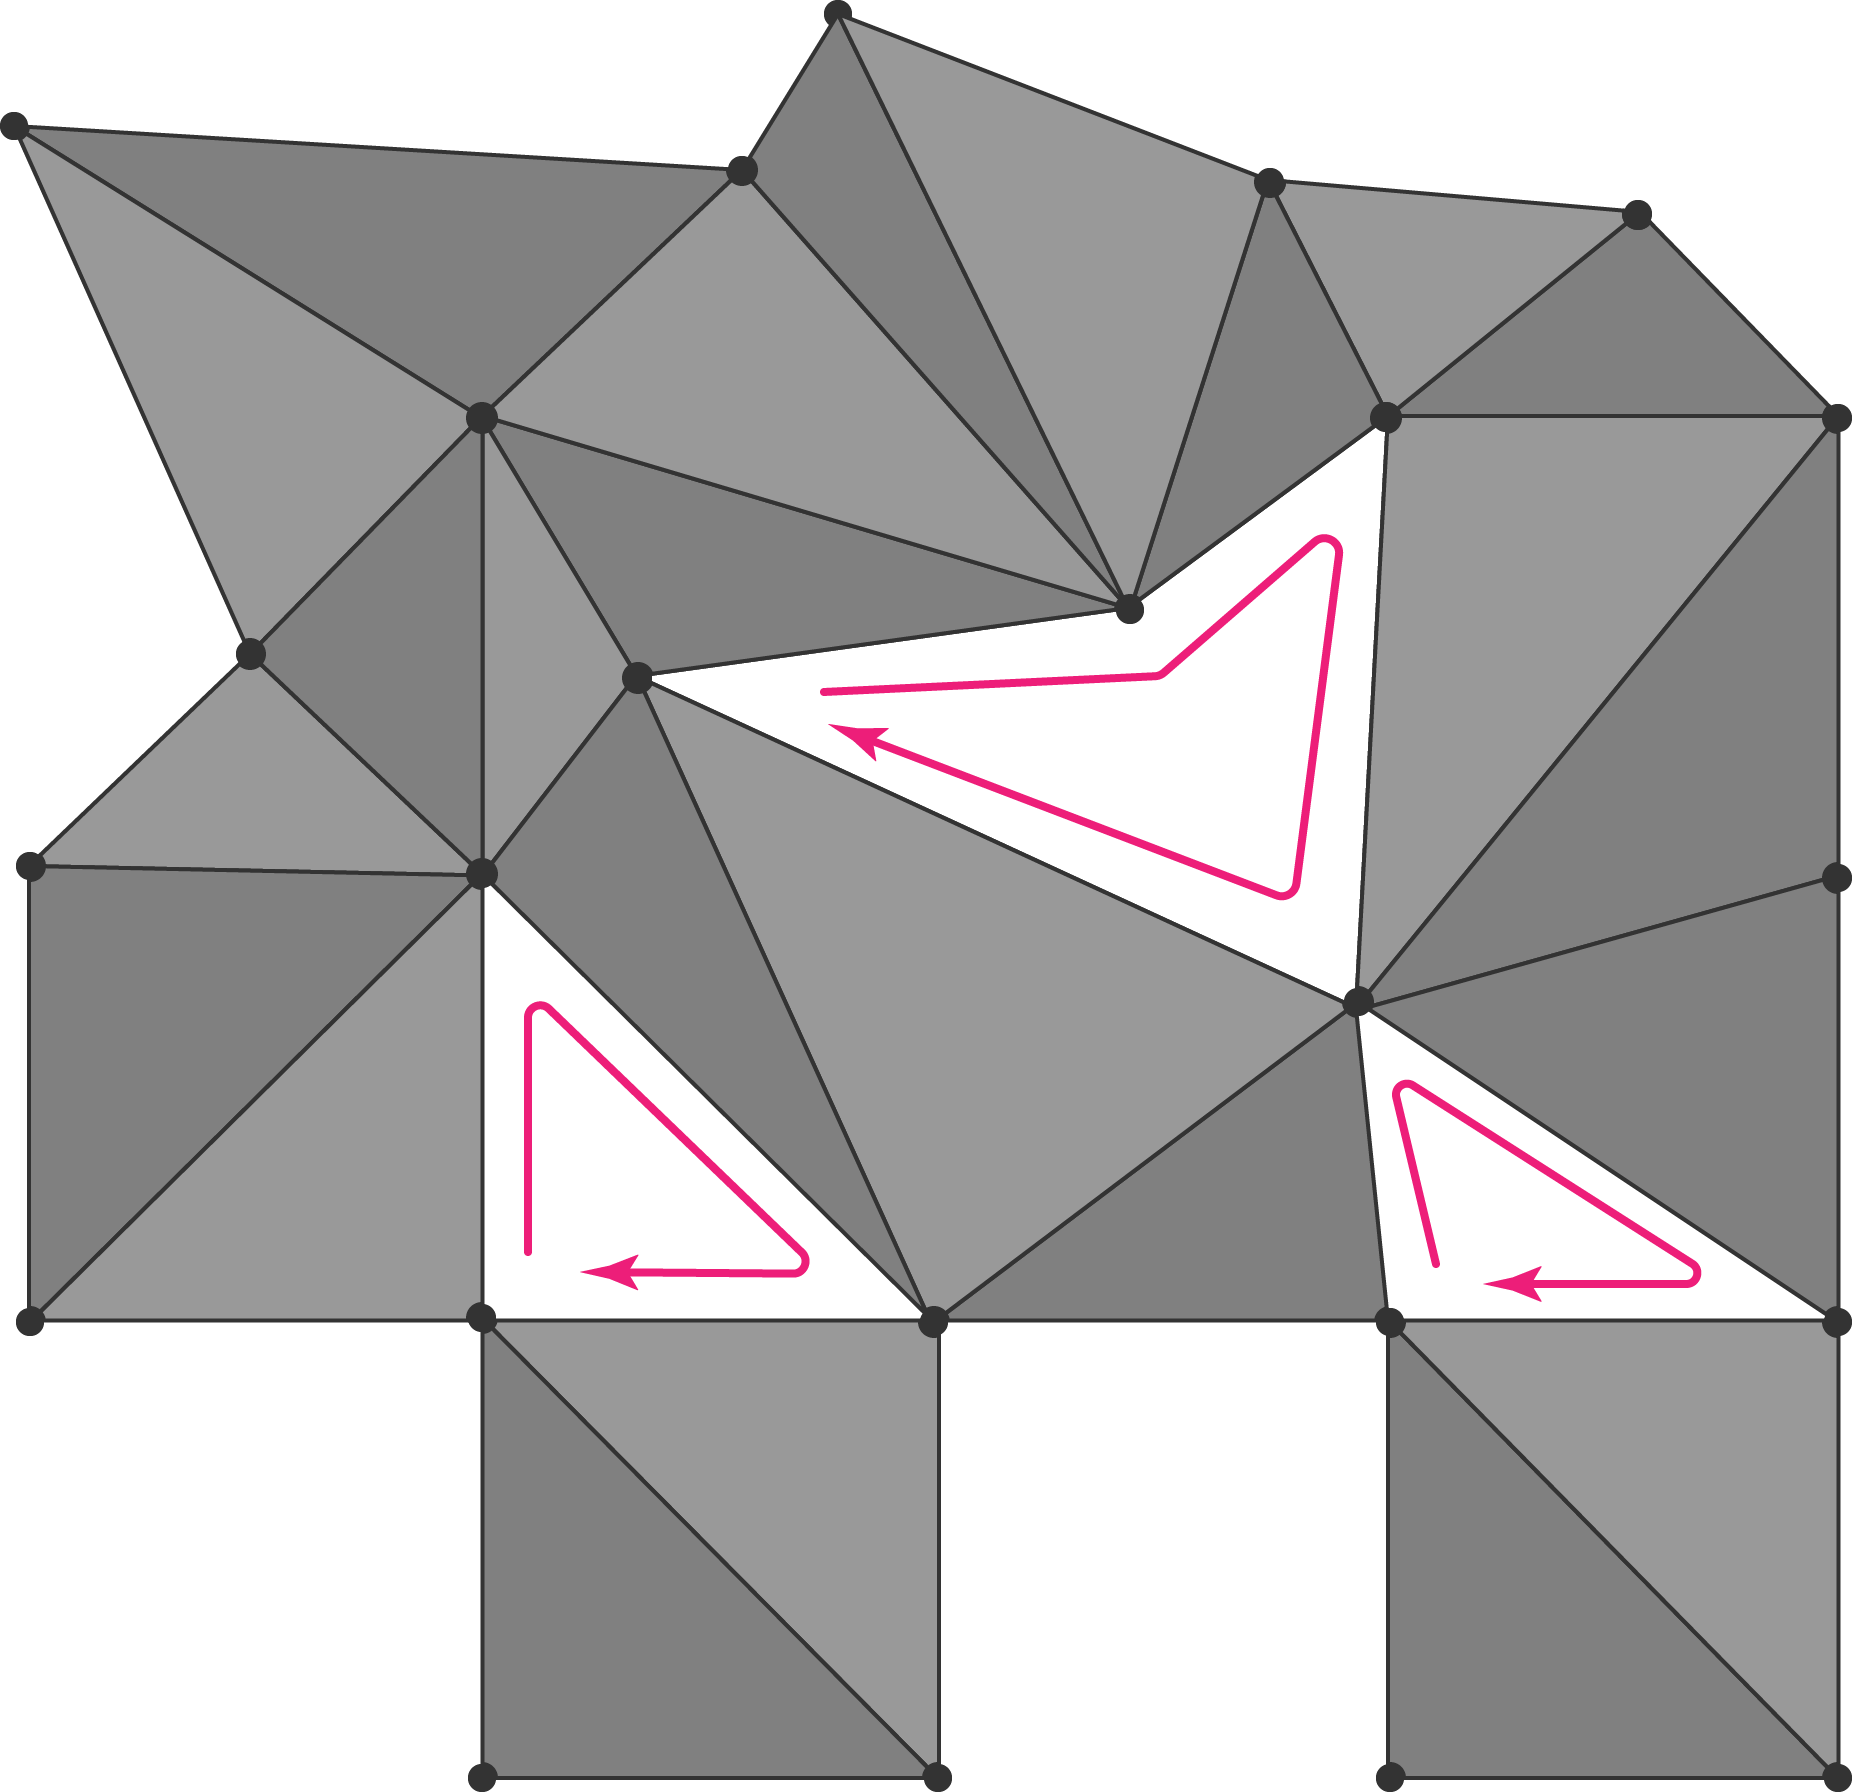
\includegraphics[width=0.9\linewidth]{images/meshloop1.png}
    \caption{An example grid mesh with 24 faces, 24 vertices,
    50 edges, three loops, a genus of 3. Indeed, one can see that
    applying these numbers into our formula gives exactly 2.}
\end{marginfigure}

The \textit{genus} would be "number of holes" in the mesh. It can be computed
by many means, for example, if we know the Euler characteristic of a mesh
as $\chi$, then $\chi = 2 - 2g$ \cite{weisstein_genus}.

For a closed (solid) model, every edge has two faces, and every face has at least
three edges, so $2e \ge 3f$. If the mesh is all triangles, as the GPU demands, then
$2e = 3f$. Assuming a genus of $0$ and substituting $1.5f$ for $e$ in the formula 
yields $f \le 2v-4$ If all faces are triangles, then $f = 2v-4$.

\begin{marginfigure}
    \centering
    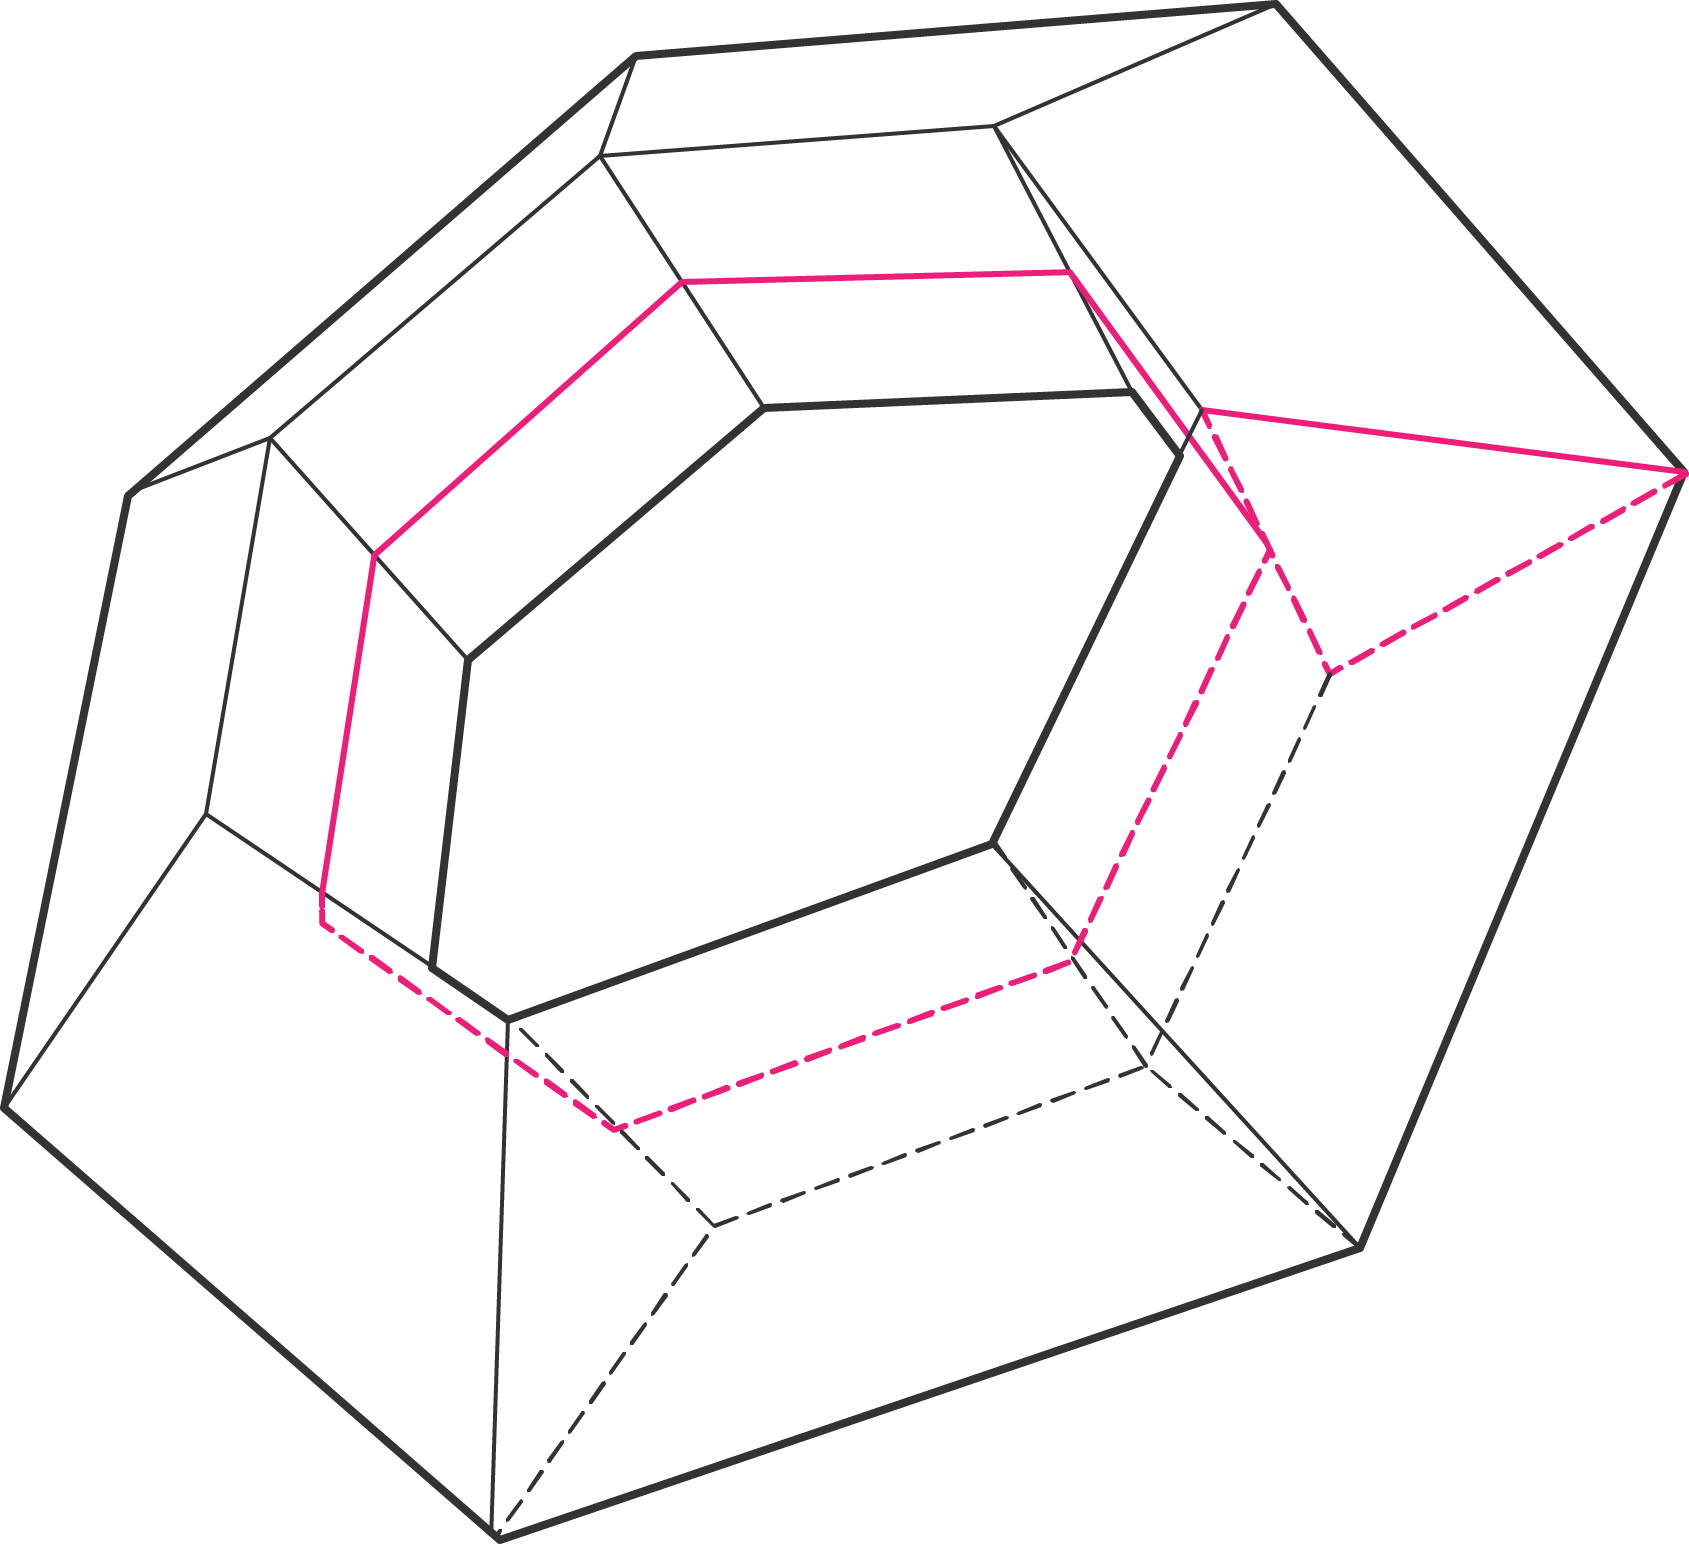
\includegraphics[width=0.8\linewidth]{images/donuttopology.png}
    \caption{A discrete torus mesh still contains many of the same topological
    properties of its continous counterparts. This can be understood in terms
    of an equivalence of graphs to the embedding diagrams of many of these figures.}
\end{marginfigure}

\section{Normals}

In 3D space, every little plane has a corresponding vector pointing
outwards out of it, orthogonally; the size of such a vector is proportional
to the size of the area of the little plane.

\begin{marginfigure}
    \centering
    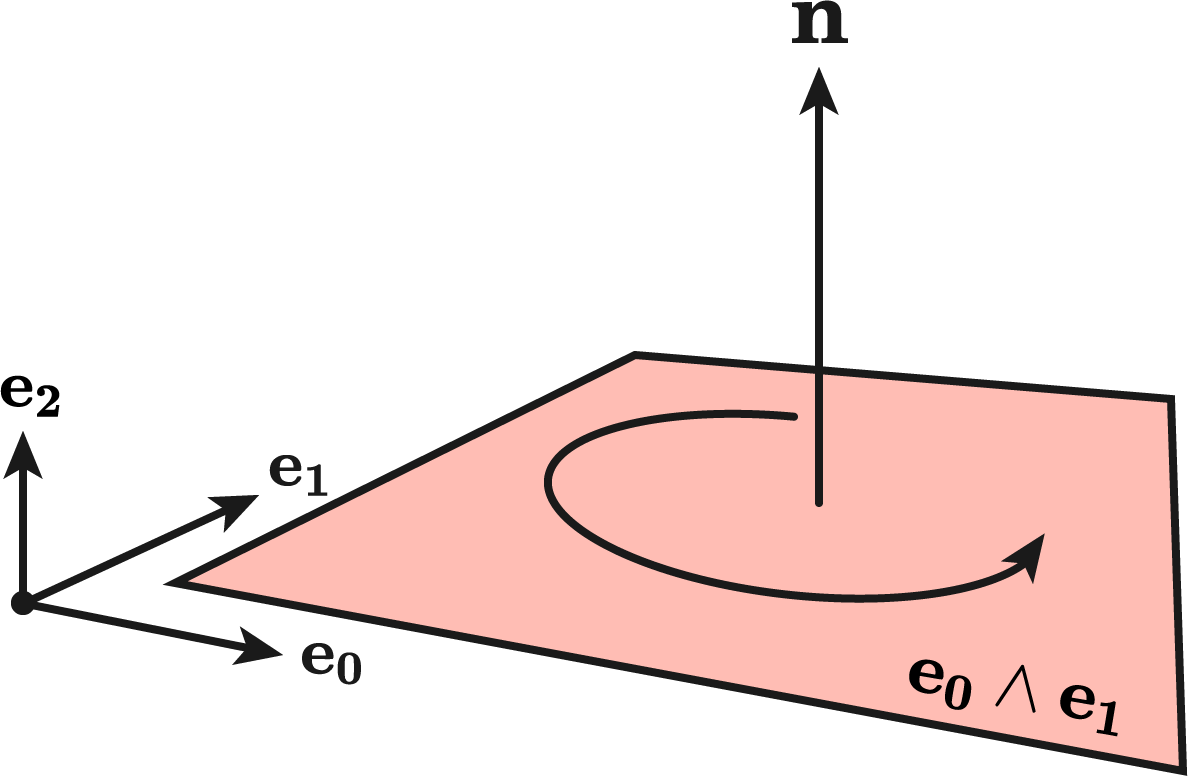
\includegraphics[width=0.7\linewidth]{images/bivectornormal.png}
    \caption{The plane represented by the bivector $\bf{B}$ generated
    by $\bf{e_0\wedge e_1}$ has a normal, axial vector 
    $\bf{n = e_0 \times e_1}$.}
\end{marginfigure}

\spa

You can make sense of this in many ways, but this is a property unique to
3D space. Using geometric algebra, one can very easily see two very
important properties that normals have, their \emph{orientation}
and the idea of \emph{normalization}. Indeed, if a mesh face or any general
plane is given by a bivector $\bf{B= a \wedge b}$, then the associated
\emph{\textbf{normal vector}} is the dual:

\begin{align*}
    \bf{n} &= \begin{pmatrix}
\text{Area of} \\
\text{plane}
\end{pmatrix}^{-1}
\begin{pmatrix}
\text{Dual of} \\
\text{said plane}
\end{pmatrix} \\
    &= |\bf{B}|^{-1} i\bf{B} \\
    &= |\bf{B}|^{-1} i(\bf{a \wedge b}) \\
\end{align*}

\spa

First, we see that normal vectors are \emph{pseudovectors} and not
real vectors. This is very important mathematically, as bivectors
(and therefore pseudovectors corresponding to said bivectors) behave
rather unusually under a given transformation matrix $\bf{M}$.
Whilst by basic linear algebra $\bf{v \rightarrow Mv}$, the
\emph{cross product}, or bivector, 
\href{https://peeterjoot.com/2024/01/21/bivector-transformation-and-reciprocal-frame-for-column-vectors-of-a-transformation/}{transforms}:

\begin{align*}
\bf{B} &\longrightarrow |\bf{M}| \bf{(B\wedge e_i) m^i} \\
 \bf{a \times b} &\longrightarrow (\text{adj } \bf{M})^T (\bf{a \times b})
\end{align*}

As pointed out in \cite{graphicscompendium},
if the surface was somehow deformed by some non-uniform scale transformation,
the rescaling matrix is not simply an inverse. This introduces all kinds
of extra complications when making algorithms for mesh deformations,
subdivision and etc, as one needs to be careful as to conserve the normals.

\subsection{Per-vertex normals / Pseudonormals} \label{per-vertex-normals}

A vertex is just a point, there is no inherent sense of direction
or magnitude associated to it; but it's convenient to want the normals
not associated to the faces, but the normals of a mesh. These are
also called \textit{pseudonormals} \cite{SDFnormal}.

\spa

So how does one do this? There are many somewhat equivalent
ways of choosing a normal. First, you have to choose a direction
relative to the vertex, and then a size. The basic idea is that
you can look at all the faces around you and their normals,
and take an average of all those normals:

\begin{definition}[Per-vertex normals]
    \begin{align*}
    (\text{Vertex normal}) = 
    \sum_{\text{Faces around vertex}} 
\begin{pmatrix}
\text{Normal vectors}\\
\text{from neighbour}\\
\text{faces to vertex}
\end{pmatrix}
\text{(Weight factor)}
\end{align*}

Which is written down normally (heh) as:

\begin{align*}
    \widetilde{\bf{n}_v} = 
    \sum_{f} \bf{n}_f w_f
\end{align*}

Where later on you just normalize the total normal
$\bf{n}_v$. 
The weight factor $w_f$ comes in three flavors of choice.
The last two are the most common:

\begin{itemize}
    \item \textbf{Uniform weighting:}
    We have that $w_f = 1$. The interpretation being that
    all face normals contribute equally to the total result.
    This "democratic principle" of vertex weighting is discussed
    below.
    
    \item \textbf{Area weighting:}
    We have that $w_f \propto A_f $, where $A_f$ is the area
    of the face. The larger the face, the more those normals
    contribute to the vertex normal.

    \item \textbf{Angle weighting:}
    We have that $w_f \propto \theta_f$, where $\theta_f$ is the
    angles subtended from the vertex to the other edges of the bounding
    faces. 
\end{itemize}
\end{definition}


\begin{marginfigure}
    \centering
    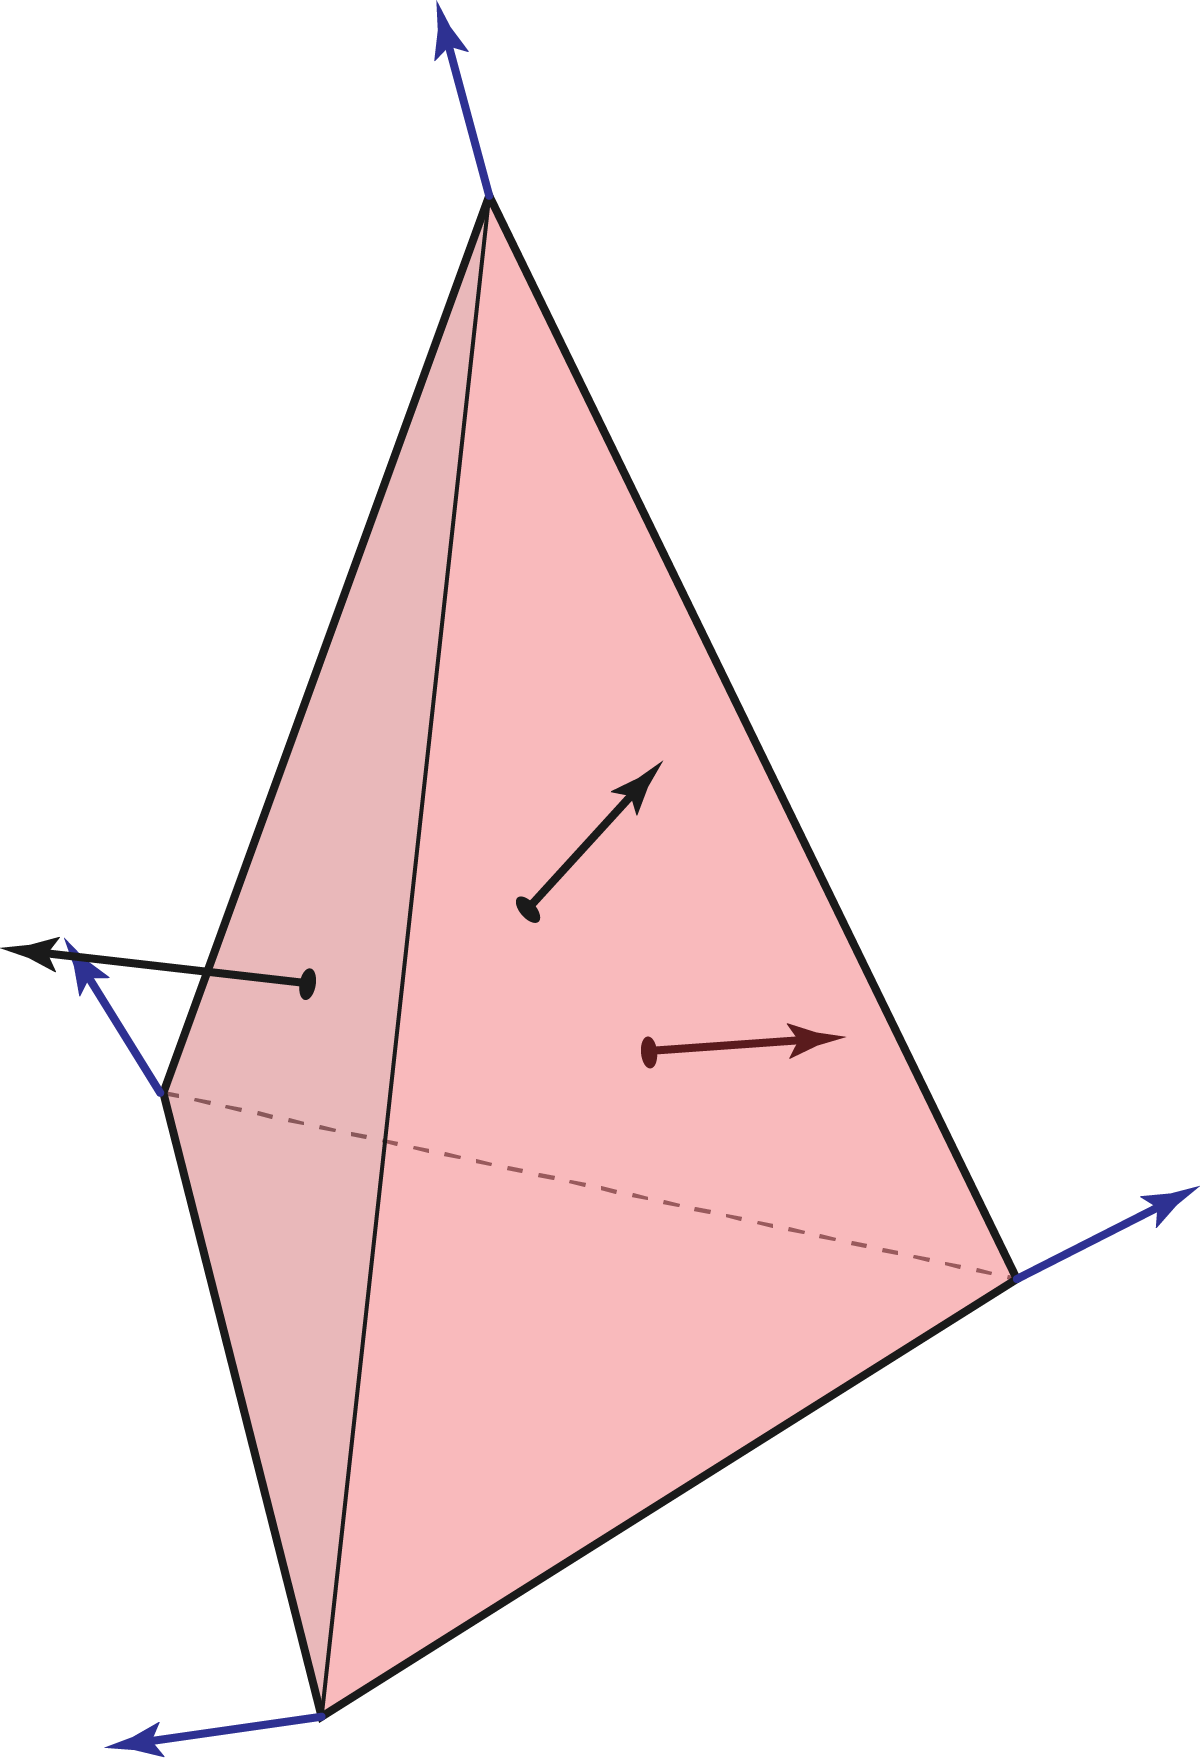
\includegraphics[width=0.8\linewidth]{images/pervertex.png}
    \caption{The face normals versus the area-weighted vertex normals
    of a simple tetrahedron without the bottom face.}
\end{marginfigure}

\spa

But why would we do these averaging procedures? Surely one can
just take all the normals around the vertex and average them
at once, like this:

\begin{align*}
    \bf{n}_v = \sum_i \bf{n}_f 
    (|\bf{n}_f|)^{-1}
\end{align*}

Not so \cite{vertex1}, one quickly
learns that if the faces around the vertex are sufficiently
distorted, even if the geometry remains the same, or that if one
adds \emph{more faces}, keeping the same geometry, one still gets
different vertex normals.

\spa

These three methods ensure that doesn't happen. The linked
paper claims the tesselation of the mesh doesn't affect the angle
method, so that would be generally better for geometric goals.

\spa

One can do a \textbf{shared normals scheme} as well, where
multiple normals can exist in the same vertex.
\section{Boundaries of Surfaces} \label{boundary}
%%https://en.wikipedia.org/wiki/Manifold#Manifold_with_boundary 


\section{Curvature} \label{curvature}

As discussed in \cite{discreteexterior1}, whilst curvature can be
easily defined in the continous setting, the discrete setting has no
trivial way of assigning curvature to surfaces due to the lack of 
differentiability and continuity in many functions. Therefore,
one can produce a \textit{array} of multiple discrete curvature
definitions, these that all approach the continous one at the
"infinite resolution" limit. For example, the basic curvature of a 
parametric curve $\gamma(s)$ is given by:

\begin{example}[Line gaussian curvature]
\begin{align*}
\kappa(s) = \frac{|| \gamma'(s) \wedge \gamma''(S) ||}{|| \gamma'(s) ||^3}
\end{align*}    
\end{example}


This scaled bivector area, a prelude to the generalized Riemann curvature,
\sidenote{The Riemman curvature is given as $\bf{Rie(a \wedge b)} = 
\partial_x \wedge \partial_y P_x(a) \cdot P_y(b)$ \cite{geometric_calculus1},
which is exactly a bivector to bivector function that maps the total
"area deficit" or "infinitesimal rotation generators" produced by local
spatial curvature. The deficit of the curve would exactly be the one
produced by its intrinsic curvature.}
gives us all the information we need, but in the discrete case, if
we're dealing with meshes and polylines, all vertex joints have
a "infinite" amount of curvature, and along the actual curve, none at all.
This can be remedied by doing a "cumulative check" over the whole arclength;
these curvature energy integrals then gives us a more \textit{global}
rather than strictly \textit{local} definition.

\begin{marginfigure}
    \centering
    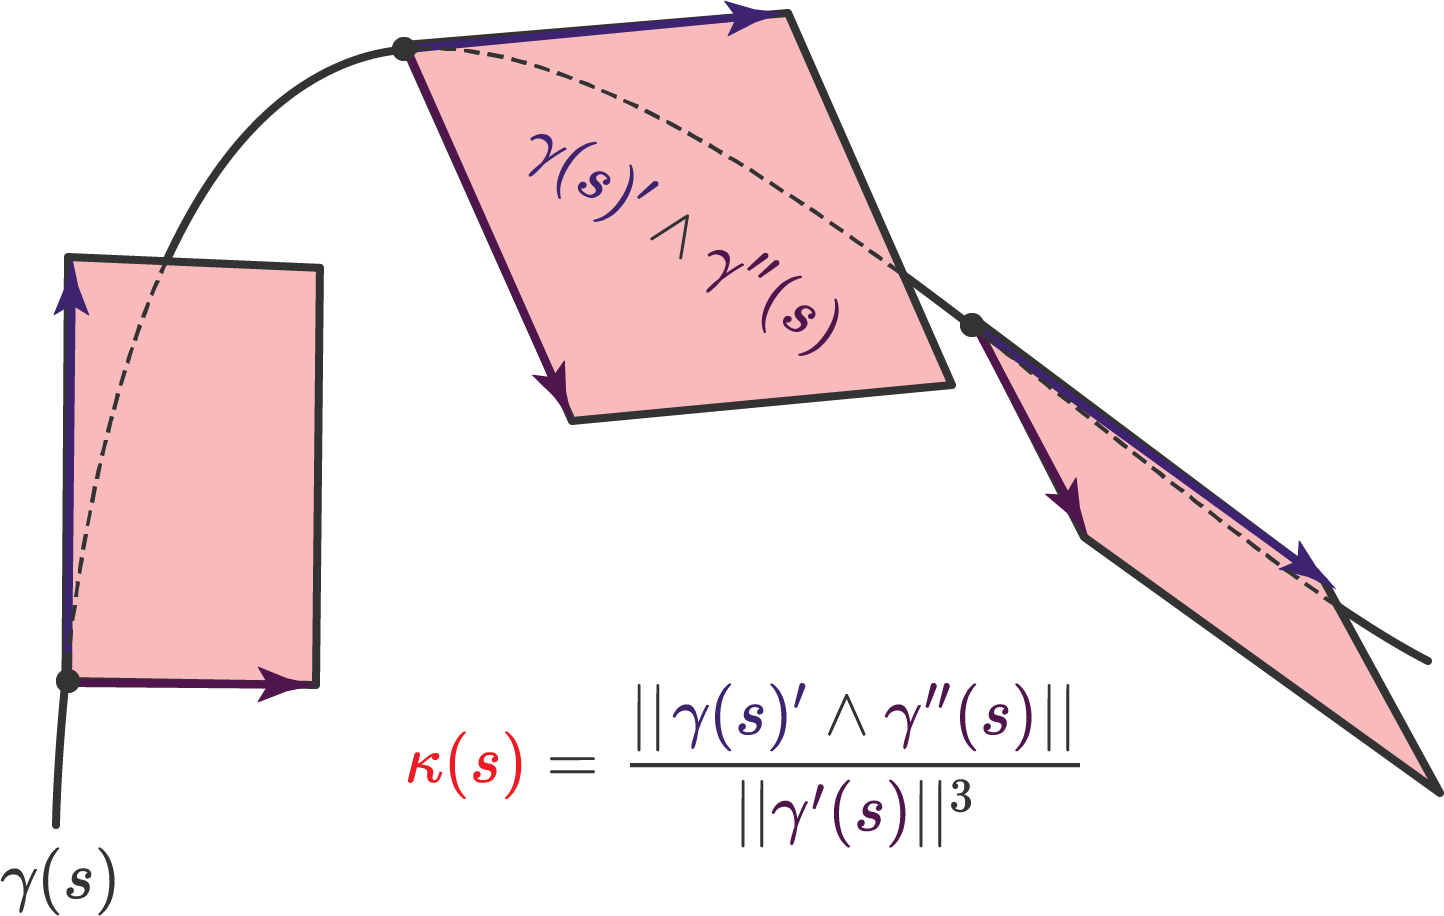
\includegraphics[width=1.0\linewidth]{images/curvature1.png}
    \caption{The curvature of a parametrized line $\gamma(s)$ is
    given by the reduced area of the bivector spanned by its velocity
    $(\gamma'(s))$ and acceleration $(\gamma''(s))$ vectors.}
\end{marginfigure}


\spa

We have four basic curvatures to deal with, \textit{\textbf{turning angle,
length variation, osculating circle}} and \textit{\textbf{Steiner's formula}},
all equivalent in the continous case, but inequivalent in the discrete one.
A complete description is in the \textit{discrete curvature 2} section of
\cite{discreteexterior1}.

\subsection{Turning angle}

The first curvature that was partially implemented in the course in
\ref{angle-defect-algorithm} was the \textit{turning angle} one, 
originally put in \cite{Crane:2010:TCD}, it approximates the associated
holonomy of edge loops along the entire mesh.

\spa

The idea is to compute two matrices, $\bf{A} = [d_0^T, \ H_{ij}^T]^T$
and $\bf{B} = [k, \ z]^T$, that give the number of contractible
and non-contractible basis cycles in a mesh, and the angle defects 
around said cycles corrected for the total Euler characteristic $\chi$
of the surface mesh.


\subsection{Riemann curvature and such}

In usual exterior calculus, the Riemann tensor is of the form
$F \approx d\bf{A} + \bf{[A,A]}$; the approximation using
discrete exterior calculus is to see variations in area/volume
in Delaunay triangulations. In \cite{exterior_calculus1},
the idea is that $\bf{Rie(a,b)}$ is:

\begin{align*}
R_v&=\frac{\sum_{h_{\mid v}} R_h A_h^* A_{h v}}{\sum_{h_{\mid v}} A_h^* A_{h v}} \\
 &=\frac{\sum_{h \mid v} R_h A_h^* A_{h v} / \sum_{h_{\mid v}} A_{h v}}{\sum_{h_{\mid v}} A_h^* A_{h v} / \sum_{h_{\mid v}} A_{h v}}
\end{align*}

\begin{align*}
\langle Q\rangle_v \equiv \frac{\sum_{h_{\mid v}} Q_h A_{h v}}{\sum_{h_{\mid v}} A_{h v}}
R_v=\frac{\left\langle R_h A_h^*\right\rangle_v}{\left\langle A_h^*\right\rangle_v}
\end{align*}

\subsection{Minimal surfaces}

A saddle is a good example of a minimal surface.
\cite{bouma2001}